\documentclass{article}\usepackage{graphicx, color}
%% maxwidth is the original width if it is less than linewidth
%% otherwise use linewidth (to make sure the graphics do not exceed the margin)
\makeatletter
\def\maxwidth{ %
  \ifdim\Gin@nat@width>\linewidth
    \linewidth
  \else
    \Gin@nat@width
  \fi
}
\makeatother

\IfFileExists{upquote.sty}{\usepackage{upquote}}{}
\definecolor{fgcolor}{rgb}{0.2, 0.2, 0.2}
\newcommand{\hlnumber}[1]{\textcolor[rgb]{0,0,0}{#1}}%
\newcommand{\hlfunctioncall}[1]{\textcolor[rgb]{0.501960784313725,0,0.329411764705882}{\textbf{#1}}}%
\newcommand{\hlstring}[1]{\textcolor[rgb]{0.6,0.6,1}{#1}}%
\newcommand{\hlkeyword}[1]{\textcolor[rgb]{0,0,0}{\textbf{#1}}}%
\newcommand{\hlargument}[1]{\textcolor[rgb]{0.690196078431373,0.250980392156863,0.0196078431372549}{#1}}%
\newcommand{\hlcomment}[1]{\textcolor[rgb]{0.180392156862745,0.6,0.341176470588235}{#1}}%
\newcommand{\hlroxygencomment}[1]{\textcolor[rgb]{0.43921568627451,0.47843137254902,0.701960784313725}{#1}}%
\newcommand{\hlformalargs}[1]{\textcolor[rgb]{0.690196078431373,0.250980392156863,0.0196078431372549}{#1}}%
\newcommand{\hleqformalargs}[1]{\textcolor[rgb]{0.690196078431373,0.250980392156863,0.0196078431372549}{#1}}%
\newcommand{\hlassignement}[1]{\textcolor[rgb]{0,0,0}{\textbf{#1}}}%
\newcommand{\hlpackage}[1]{\textcolor[rgb]{0.588235294117647,0.709803921568627,0.145098039215686}{#1}}%
\newcommand{\hlslot}[1]{\textit{#1}}%
\newcommand{\hlsymbol}[1]{\textcolor[rgb]{0,0,0}{#1}}%
\newcommand{\hlprompt}[1]{\textcolor[rgb]{0.2,0.2,0.2}{#1}}%

\usepackage{framed}
\makeatletter
\newenvironment{kframe}{%
 \def\at@end@of@kframe{}%
 \ifinner\ifhmode%
  \def\at@end@of@kframe{\end{minipage}}%
  \begin{minipage}{\columnwidth}%
 \fi\fi%
 \def\FrameCommand##1{\hskip\@totalleftmargin \hskip-\fboxsep
 \colorbox{shadecolor}{##1}\hskip-\fboxsep
     % There is no \\@totalrightmargin, so:
     \hskip-\linewidth \hskip-\@totalleftmargin \hskip\columnwidth}%
 \MakeFramed {\advance\hsize-\width
   \@totalleftmargin\z@ \linewidth\hsize
   \@setminipage}}%
 {\par\unskip\endMakeFramed%
 \at@end@of@kframe}
\makeatother

\definecolor{shadecolor}{rgb}{.97, .97, .97}
\definecolor{messagecolor}{rgb}{0, 0, 0}
\definecolor{warningcolor}{rgb}{1, 0, 1}
\definecolor{errorcolor}{rgb}{1, 0, 0}
\newenvironment{knitrout}{}{} % an empty environment to be redefined in TeX

\usepackage{alltt}
\usepackage{times}
\usepackage{ie07}
\usepackage{hyperref}





\begin{document}


\title{AN OPEN SOURCE TOOL TO ESTIMATE MASS AND EFFICIENCY OF WIND TURBINE POWER TAKE-OFF SYSTEMS}

\authorname{Ozan Keysan, Markus A. Mueller}
\authoraddr{Institute for Energy Systems, University of Edinburgh, EH93JL, U.K.\\
Email: o.keysan@ed.ac.uk}

\maketitle

\keywords
Wind turbine, mass estimation, direct-drive, gearbox, generator

\abstract
This is where the abstract should be placed. It should
consist of one paragraph and a concise summary of the
material discussed in the article below. It is preferable not
to use footnotes in the abstract or the title. The
acknowledgement for funding organisations etc. is placed
in a separate section at the end of the text. We wish you
success with the preparation of your manuscript.

\section{Introduction}

Far offshore wind turbines can help to exploit the wind energy resources that remained untapped so far. These turbines tend to be installed as floating platforms. Reliability and mechanical stability is one of the most important issues of floating wind turbines. The nacelle mass is critical for the mechanical stability of the platform. A heavy nacelle requires larger ballast and increases the installation cost. The type of the power take-off system has a direct effect on the nacelle mass. Although, doubly-fed induction generator coupled to a multi-stage gearbox configuration is the mostly preferred for onshore wind turbines; it may not be the most suitable option for a large offshore wind turbine.

Figure 1- Mass variation of three-stage wind turbine gearboxes as a function of the input torque.
In this study, a design tool is developed to estimate the mass and efficiency of various power take-off (PTO) systems of a wind turbine. Data from manufacturers and literature are collected to obtain mass and efficiency trend lines for wind turbine components. For example, Figure 1 presents the mass variation of a three stage gearbox as a function of the input torque. The components covered at the moment are gearbox, generator, bearing and shaft. It is planned to add nacelle and blade mass estimation to the full paper submission. The generator types covered are induction generator, permanent-magnet generator, synchronous generator and superconducting generator. The cooling method for the generators are also defined (air or water cooled). 
All these data are combined in an open-source design tool. The user can select different PTO systems, and then define the input power and rotational speed The design tool gives the mass and efficiency of the components. Thus, it is very easy for a user to compare different PTO systems and modify the mechanical models based on these estimations. The design tool is built using Matlab GUI. The aim of the study is to publish it as a web application that is open to wind turbine designers. We aim to expand the toolbox for the reliability calculation of the different PTO systems. The design tool will help the designers to compare different PTO systems and select the most suitable option for the specific application.


\begin{knitrout}
\definecolor{shadecolor}{rgb}{0.969, 0.969, 0.969}\color{fgcolor}\begin{figure}[]

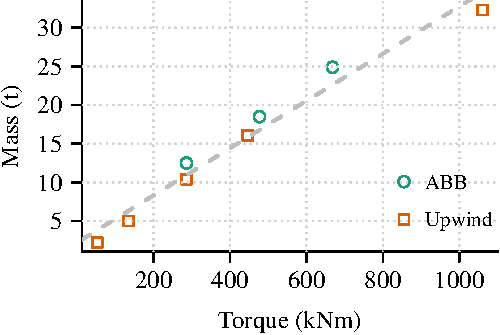
\includegraphics[width=\maxwidth]{figure/plot1gpm} \caption[Mass of the medium speed permanent magnet gnenerator vs torque]{Mass of the medium speed permanent magnet gnenerator vs torque.\label{fig:plot1gpm}}
\end{figure}


\end{knitrout}


As shonw in \autoref{fig:plot1gpm}

The proceedings for IE 07 will contain all the accepted
papers following the peer review process. Authors are
asked to prepare and submit the {\bf PDF} electronic versions
of their full papers according to the instructions below.

\section{Manuscript preparation}
Full papers must be typed in English. The title of the
paper is typed in CAPITAL LETTERS (boldface 18pt)
and centred on the page. The author's name is typed in
capital and lower case bold letters and centred on the
page. Directly under the author's name in capital and
lower case letters and also centred is the author's
affiliation, address, plus e-mail address and fax number of
(at least) the corresponding author. Manuscripts must be
typed single spaced using 10 point characters. Only
Times, Times Roman, Times New Roman and Symbol
fonts are accepted. The text should be typed on an A4
paper (21 cm x 29.7 cm). The paper should have margins
of 2.4 cm from top and bottom and 2 cm from left and
right. Paragraphs are separated by 6 points and with no
indentation. The text of the full papers is written in two
columns and justified. Each column has a width of 8.3 cm
and the columns are separated by a margin of 0.4 cm. The
maximum length of the full paper is 8 pages, of the short
and the demo paper 4 pages. Do not number the pages.
The final format in which the papers will appear on the
CD ROM will be a PDF file. Authors are requested to send
a PDF file of their final paper to be included directly
in the CD ROM.

\subsection{Figures and tables}
Figures and tables should be centred in the column,
numbered consecutively throughout the text, and each
should have a caption underneath it (see for example
Table~\ref{tab1}). Care should be taken that the lettering
is not too small. All figures and tables should be included
in the electronic versions of the full paper.


\begin{table}[htb!]
\begin{center}

\begin{tabular}{|l|l|}
\hline
{\em n} & {\em n!} \\
\hline
1 & 1  \\
2 & 2  \\
3  & 6\\
\hline
\end{tabular}
\end{center}
\caption{\label{tab1}This is an example of a table caption.}
\end{table}

\subsubsection{Equations}
Equations should be typed within the text, centred, and
should be numbered consecutively throughout the text.
They should be referred to in the text as Equation (n).
Their numbers should be typed in parentheses, flush right,
as in the following example.
\begin{equation}
	    PA + A'P - PBR^{-1}B'P + Q  =  0 \enspace.
\end{equation}

\subsubsection{References}
The list of references should be ordered alphabetically
according to the first author surname. All references
should be cited in the text, and using square brackets such
as \cite{ref01} and \cite{ref02}.

\section{Generating a {PDF} file}
The PDF format will be the final format under which the
papers will appear in the {CD ROM}. You {\bf SHOULD}
submit your paper as {PDF} document.

\section{Electronic submission of the full paper}
You should submit your {PDF} file which should adhere to
the above format via the conference paper submission
system.

\section*{Acknowledgements}
The acknowledgement for funding organisations etc.
should be placed in a separate section at the end of the
text. Thank you for your cooperation in complying with
these instructions.

\bibliography{ie07}
\noindent
\bibliographystyle{plain}

\end{document}
